\subsection{V3: нагрев пара только через ТВЭЛ}

По требованию физической постановки V3 исключает отдельный нагреватель пара. Вся энергия вводится в топливо GeN-Foam через \texttt{nuclearFuelPin}, затем проходит через топливо, зазор, W-оболочку и только после этого попадает в локальный водный слой. Python-часть больше не задает долю импульса, дошедшую до воды. Она интегрирует поток от наружной стенки:
\[
\frac{dE_w}{dt} = h_{\mathrm{eff}} A_{\mathrm{об}}
\max(T_{\mathrm{об}}-T_w,0),
\qquad
T_w \le T_{\mathrm{об}}.
\]
Коэффициент \(h_{\mathrm{eff}}\) выбирается по текущей фазе воды: однофазный нагрев, кипение или перегретый пар; в сухом паре добавляется радиационная поправка W-стенка--пар. Поэтому модель проверяет именно вопрос: может ли нагретый ТВЭЛ сам довести воду или пар до \(T^*_{\mathrm{дис}}\), не разрушая топливо и оболочку.

\begin{figure}[H]
    \centering
    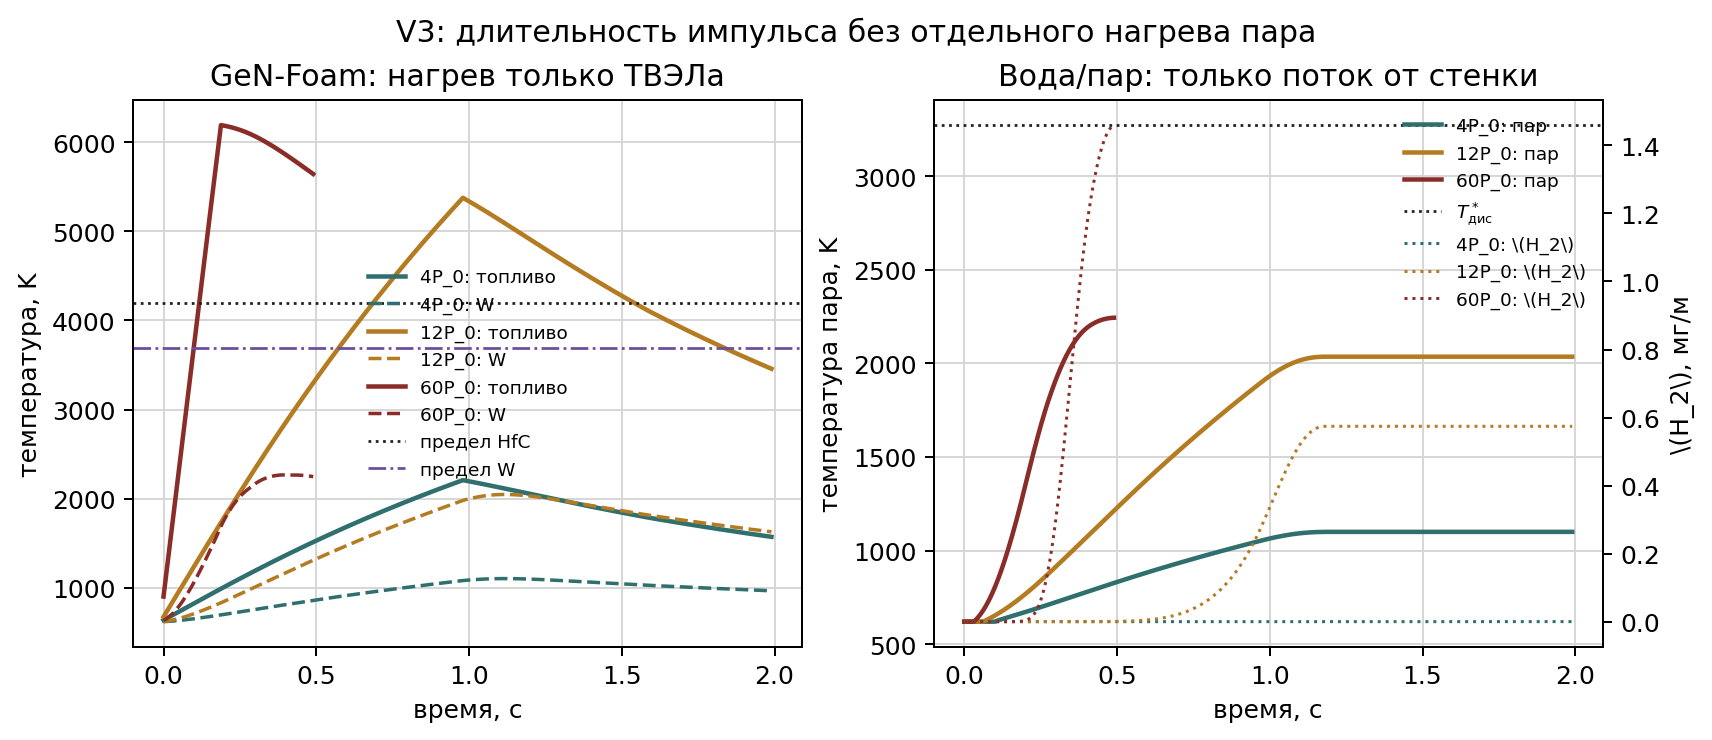
\includegraphics[width=0.88\textwidth]{figures/pipeline_v3_tvel_heating.png}
    \caption{V3 без отдельного нагрева пара: GeN-Foam греет только ТВЭЛ, а вода получает энергию через наружную W-оболочку. Длинный импульс улучшает теплопередачу, но в текущей геометрии целевое паровое окно не открывается без перегрева топлива.}
    \label{fig:pipelineV3TvelHeating}
\end{figure}

\begin{table}[H]
    \centering
    \caption{Проверка гипотезы о длительности импульса для нагрева пара через ТВЭЛ.}
    \label{tab:pipelineV3TvelHeating}
    \footnotesize
    \resizebox{\textwidth}{!}{%
    \begin{tabular}{@{}p{4.0cm}rrrrrrrp{4.8cm}@{}}
    \hline
    Сценарий & \(\tau_p\), с & \(P/P_0\) & \(T_f^{\max}\), K & \(T_W^{\max}\), K & \(T_s^{\max}\), K & \(\eta_s\), \% & \(m_{H_2}\), мг/м & Вывод \\
    \hline
    \(HfC\)--W, \(4P_0\), \(1.0\,\mathrm{s}\) & 1.00 & 4 & 2208 & 1105 & 1100 & 0.0955 & \ensuremath{1.250\cdot10^{-4}} & пределы соблюдены, но паровое окно не достигнуто \\
\(HfC\)--W, \(12P_0\), \(1.0\,\mathrm{s}\) & 1.00 & 12 & 5374 & 2048 & 2036 & 0.0648 & 0.574 & реакторная часть перегрета до достижения парового окна \\
\(HfC\)--W, \(60P_0\), \(0.2\,\mathrm{s}\) & 0.20 & 60 & 6190 & 2267 & 2244 & 0.0722 & 1.460 & реакторная часть перегрета до достижения парового окна \\
    \hline
    \end{tabular}
    }
\end{table}

Расчет показывает, почему простое увеличение длительности импульса не является автоматическим решением. Более длинный импульс действительно дает теплу больше времени пройти к W-оболочке и водному слою, но температура пара остается ограничена температурой наружной стенки. В коротком жестком импульсе топливо перегревается раньше, чем оболочка и пар достигают области диссоциации. В растянутом импульсе теплопередача мягче, но целевой уровень \(T_s\approx3273\,\mathrm{K}\) все равно не достигается. Следовательно, в текущей геометрии одного ТВЭЛа положительный водородный режим через один только нагрев топлива не получается; для продолжения нужны не отдельный нагреватель пара, а изменение самой теплопередающей геометрии ТВЭЛа, например уменьшение теплового сопротивления зазора, другой радиус/толщина активного слоя или отдельная квалифицированная стенка горячего канала.
